\documentclass{ximera}
%\usepackage{tkz-euclide,tikz}
\title{Feature test}

\begin{document}
\begin{abstract}
    Testing of features
\end{abstract}
\maketitle

%% \begin{sagesilent}
%%     p2f1 = 3*x+1
%%     p2ans = p2f1(x=4)
%% \end{sagesilent}
%% \begin{problem}
%% Let $f(x) = \sage{p2f1}$. Then $f(4) = \answer{\sage{p2ans}}$
%% \end{problem}

\begin{image}
  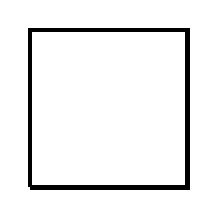
\begin{tikzpicture}
    \draw[ultra thick] (0,0) -- (2,0) -- (2,2) -- (0,2) -- (0,0);
     \end{tikzpicture}  
\end{image}


\begin{center}
    \geogebra{XC3FXUdJ}{800}{600}%%https://www.geogebra.org/m/XC3FXUdJ
\end{center}

This is a test! ANOTHER

\begin{center}
  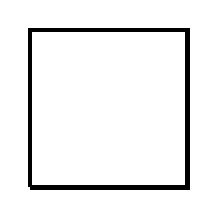
\begin{tikzpicture}
 \draw[ultra thick] (0,0) -- (2,0) -- (2,2) -- (0,2) -- (0,0);
  \end{tikzpicture}
\end{center}

\begin{onlineOnly}
\begin{center}
\desmos{f95viwzyer}{800}{600}
\end{center}
\end{onlineOnly}


\end{document}
